\section{Evaluation\label{chap:evaluation}}
To see whether the desired capabilities are fulfilled \lare{} is tested based on a sample web application.
It provides different types of pages which are designed to perform the different aspects of this evaluation.
\\
As stated in \cite{palomaki2010web} \enquote{proper test definition, execution, reporting and repeatable test results are of utmost importance}.
To achieve those criteria we focus on the test definition first.
\\
To evaluate \lare{} we first test it's functionality.
We check if the desired content is delivered and if \lare{} is performing as expected.
\\
It is not easy to test \ajax{} \webApplication{}s.
As seen in \cite{marchetto2007testing} there is a lack of good testing tools, especially when it comes to white-box testing.
\selenium{}\footnote{http://www.seleniumhq.org/} is mentioned as a good tool for black-box testing.
Also in \cite{lundmarkautomatic} it is referred to as a good possibility to test web applications.
It is also suggested in \cite{palomaki2010web} for non-abstract HTTP request performance testing, which can represent the requests of a single user.
\\
In \cite{marchetto2008state} a new automated testing technique is introduced, again based on \selenium{}.
\\
We use \selenium{} to check if \phpLare{} in combination with \twigLare{} and \lareJS{} works as expected.
In particular, we check if the same content is rendered through \lare{} as through normal \httpRequest{}s.
\\
\selenium{} additionally makes it possible to use different \webdriver{}s, in this thesis Mozilla Firefox\footnote{\url{https://www.mozilla.org/de/firefox/new/}} and Google Chrome\footnote{\url{https://www.google.de/chrome/browser/desktop/}} are used.
This is important because of the different implementations of browsers' features.
\\
To test the performance, we will use two technologies.
First of all \curl{} based tests are done.
Those tests focus on the initial request containing the markup and \lare{} requests containing the according changes.
\\
Additionally the \webApplication{} is benchmarked by using \selenium{} in combination with the \emph{window.performance} attribute, introduced in HTML5.
This method provides the possibility to check whether further requests for scripts, images, etc. are influenced.
It will show the actual load time the user has to wait, until the whole page is loaded and ready to be displayed.
\\
To design the tests as representative as possible caching in the relevant layers is enabled and disabled to see whether it influences the results or not.
Hardware and especially hard drive caching will stay untouched in our benchmarks.
\\
Mysql's caching method Query Caching will be enabled and disabled.
Twig allows template caching, which is enabled and disabled as well.
Additionally all tests are performed on a local machine and a remote server, to see whether the latency takes effect in the performance of \lare{}.
\\
We distinguish between static pages without database queries and dynamic pages containing those.
Every page relevant for the test is requested in different modes.
First of all every site will be requested normally.
After that it is requested with \lare{} enabled.
As \lare{} should only influence subsequent requests, every page will be tested with \http{} headers from different sources, imitating those requests.

%As one traditional testing model, we will evaluate the \pjaxr{} sample application via blackbox tests.
%Testing \ajax{} is not trivial due to multiple programming- and markup-languages influencing it. 
%With this tool it is possible to generate automated tests for web applications.
%
%To evaluate whether the application is crawlable or not is an important criteria whether \pjaxr{} fulfills it goals.
%Finding all the content delivered in all different URLs in the sitemap should be the target to acquire.
%The crawled content should be similar to a non-dynamic HTML file, defined for every URL.
%Content which is not directly provided via an URL but asynchronously, like via an autocompletion, should not be relevant.
%
%One way to crawl \ajax{} web applications, recommended in \cite{mesbah2012crawling} is to use Crawljax\footnote{http://crawljax.com/}. 
%It explores \ajax{}-based web applications by following every link recursively and saving the associated content. In this thesis the three endpoints of the sample project will be crawled by Crawljax to see whether all endpoints provide the same content or not.
%
%Another way to evaluate whether \pjaxr{} fulfils its goals, is testing if the Googlebot\footnote{http://google.com/bot.html} will discover all the content provided.
%Again, all three endpoints will be tested to check, if all data is found by this technique.
%While Crawljax is intended to find not easily accessible content, Googlebot is intended to find content, matching design patterns\footnote{https://developers.google.com/webmasters/ajax-crawling/} by Google. This fact makes it more challenging for \pjaxr{}, not implementing these, to have good results in this test.


\subsection{Sample web application}

The sample web application used to test \lare{} in this thesis is implemented in PHP.
To implement \lare{} we use \lareJS{} in the frontend, \twigLare{} and \phpLare{} for the backend.
\\
We use the MVC design pattern but follow the naming of django\footnote{https://docs.djangoproject.com/en/1.8/faq/general/\#django-appears-to-be-a-mvc-framework-but-you-call-the-controller-the-view-and-the-view-the-template-how-come-you-don-t-use-the-standard-names}.
\\
Instead of using models for this benchmark, we are using raw SQL queries to ensure the same queries are made every time.
Nevertheless, it is prepared to inherit from the BaseModel class to create models for later presentation purposes.
\\
The sample web application consists of two static pages \emph{/home/} and \emph{/imprint/}.
\\
To demonstrate dynamic content, we use the Delicious Dataset\footnote{http://fabianabel.de/data/mypes-www2010.html}.
This is available under \emph{/tags/}, seen in fig. \ref{fig:lare_tags}.
\begin{figure}[H]
\centering 
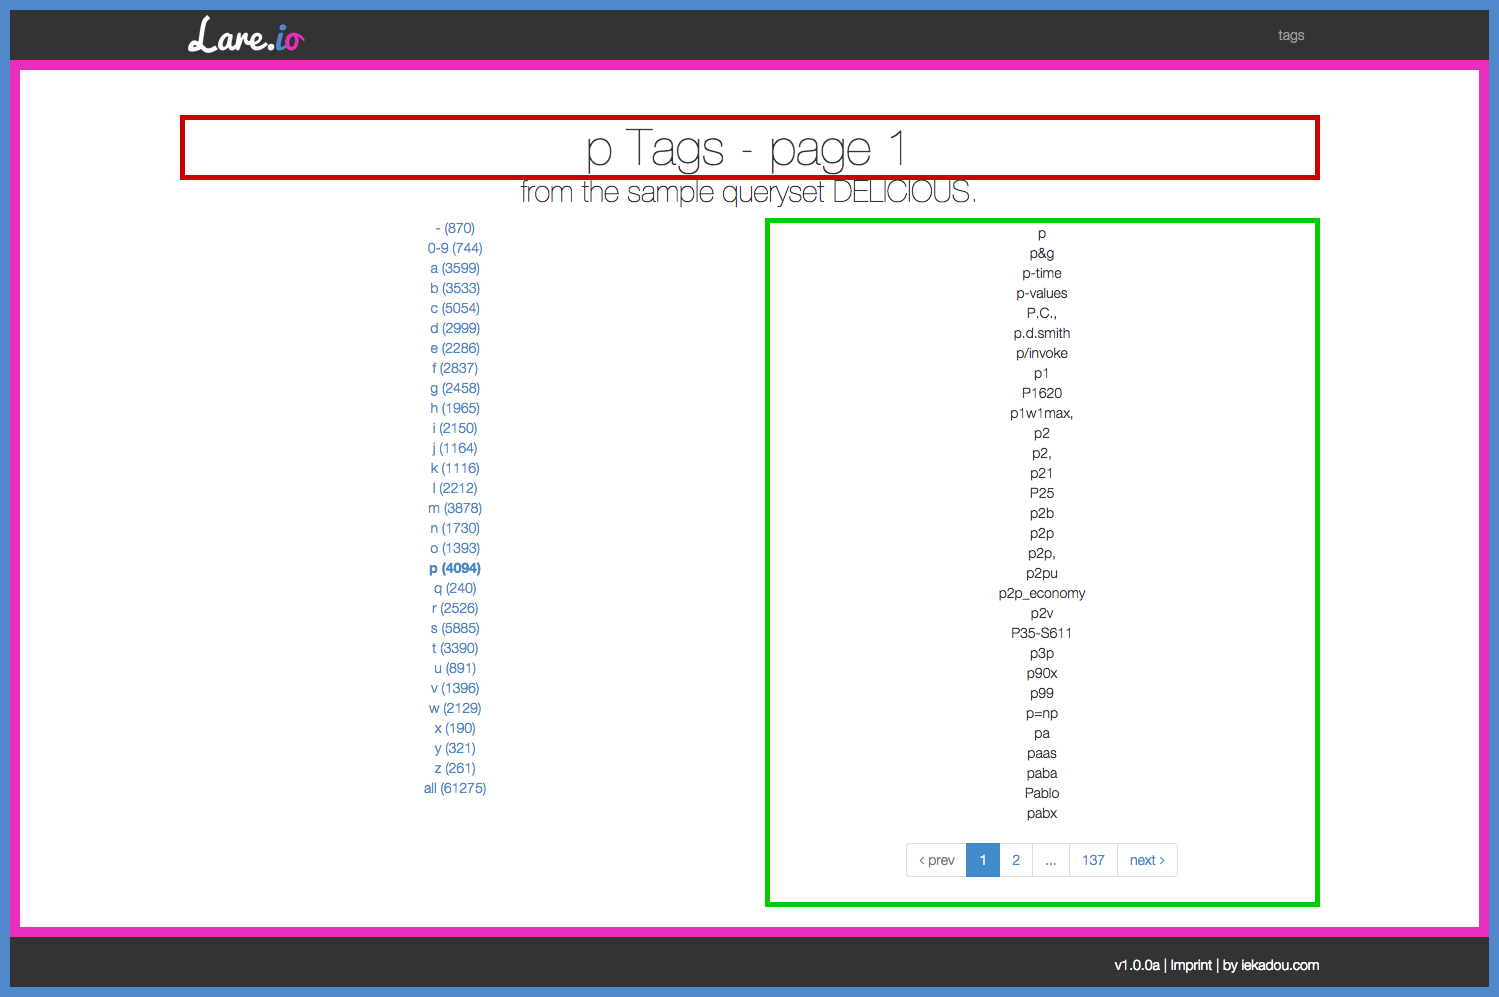
\includegraphics[width=14cm]{images/lare_p_1.png}
\caption[lare_tags]{Screenshot of /tags/p/1/ of the sample \webApplication{}}
\label{fig:lare_tags}
\end{figure}

\noindent{}On the left side of this page is a list to sub pages where the tags are categorized by it's starting character.
One of those pages exists for every alphabetic character, additionally one for tags starting with numbers and one for tags starting with non alphanumeric characters.
Behind each \emph{category} the count of tags in this category is displayed.
This list is available on every sub page under the \emph{/tags/} URL.
\\
On the right side a paginated list of all distinct tags in the current category is shown.
It is sorted alphabetically and 30 tags per page are displayed.
\\
We are using the namespaces like shown in tab. \ref{tab:sampleapp_namespaces}.

\begin{table}[h]
\centering
\begin{tabular}{llll}
	\hline
	\textbf{URL} & \textbf{Site} & \textbf{Page} & \textbf{Content} \\
	\hline
	/ & Lare & Home &  \\
	/imprint/ & Lare & Imprint &  \\
	/tags/ & Lare & Tags & all1 \\
	/tags/a/ & Lare & Tags & a1 \\
	/tags/a/ & Lare & Tags & a2 \\
	/tags/.../ & Lare & Tags & ... \\
	\hline
\end{tabular}
\caption{Namespaces of the sample web application}
\label{tab:sampleapp_namespaces}
\end{table}


\subsection{Capability tests\label{browser_functionality_tests}}

\lare{} must fulfil some requirements.
As \lare{} is divided in a frontend and a backend, we decided to write external tests to check if it works as desired.
For this purpose we use the sample \webApplication{} in combination with \selenium{}.
\\
The following capabilities are tested:
\begin{itemize}
\item Content of the response of common \httpRequest{}s
\item Content of the response of \lare{} requests
\item Back functionality
\item Forward functionality
\item URL changes when using \lare{}
\end{itemize}


\subsection{Performance Testsuite\label{testsuite}}

To test the performance of \lare{} a few different types of requests are needed to benchmark.
The reference level is a normal \httpRequest{} to each \webPage{}.
Additionally we built a \webApplication{} based on AngularJS, to have a reference of a \clientSideMVC{}.
\\
The tested pages are available at the paths:

\begin{itemize}
\item /
\item /imprint/
\item /tags/p/1/
\item /tags/p/2/
\end{itemize}

\noindent{}Additionally the \webPage{}s are requested via \lare{}.
To achieve this at \curl{} we extend the request's header with the corresponding \emph{HTTP-X-LARE} namespace.
\\
With \selenium{} we later test the pages with real web browsers to get results which are closer to reality.
The tested page to page requests are:

\begin{itemize}
  \item Self:
    \begin{itemize}
      \item / to /
      \item /imprint/ to /imprint/
      \item /tags/p/1/ to /tags/p/1/
      \item /tags/p/2/ to /tags/p/2/
    \end{itemize}
  \item Static page matching Site-Namespace:
    \begin{itemize}
      \item / to /imprint/
      \item /imprint to /
    \end{itemize}
  \item Dynamic page matching Site-Namespace:
    \begin{itemize}
      \item / to /tags/p/1/
      \item /imprint/ to /tags/p/1/
    \end{itemize}
  \item Dynamic page to static page:
    \begin{itemize}
      \item /tags/p/1/ to /
      \item /tags/p/2/ to /
      \item /tags/p/1/ to /imprint/
      \item /tags/p/2/ to /imprint/
    \end{itemize}
  \item Dynamic page matching Page-Namespace:
    \begin{itemize}
      \item /tags/p/1/ to /tags/p/2/
      \item /tags/p/2/ to /tags/p/1/
    \end{itemize}
\end{itemize}

\subsection{\curl{} benchmarks\label{curl}}
We are using \curl{} to test the plain load times of the initial request of common \httpRequest{}s and \lare{} requests.
Those \curl{} requests do not include additional data like images, scripts and stylesheets, just the plain initial HTML.
There is no point in testing the AngularJS application with this method, because the result of this request would not be the full site, since multiple \ajax{} initiated requests are needed.
\\
The bash script \enquote{curl\_tests.sh} provides the functionality to run those \curl{} tests.
To use it run:
\\
\\
\large{\textbf{{../evaluation/curl/curl\_tests.sh URL MAX\_RUNS CACERT}}}
\\
\\
\begin{tabular}{|p{4cm}|p{9cm}|}
    \hline
    \textbf{name} & \textbf{description} \\
    \hline
    URL & specifies where the web application is available, e.g. \emph{http://lare.iekadou.com} \\
    \hline
    MAX\_RUN & specifies how many times the curl requests per URL and caching settings are made. \\
    \hline
    CACERT & (optional) path to the CACERT file if necessary. \\
    \hline
\end{tabular}
\\
\\
\noindent{}To test all relevant sites we defined a variable PAGES inside the script, containing the requested paths.
For each page of those we make a normal request, followed by a \lare{} request, with the namespace defined in NAMESPACES at the same index as the PAGE which gets requested.
To get better test results we repeat those two requests \emph{MAX\_RUN} times. The output represents the load times needed in seconds.
\\
For the results in this thesis, we use a Macbook Pro Retina Early 2013 (2,7 GHz, 16GB Ram).
As web server we are running an Apache via Mamp Pro 3.1 for Mac OSX with PHP 5.3.6.
As database server we are using MySQL in version 5.5.42.
\\
Additionally we test every request with database caching (DC) enabled, disabled and template caching (TC) enabled and disabled.
\\
Local tests are run from the same machine, external tests are run from an external network to imitate behaviour like in the WWW.

\subsubsection{Results}

The following table \ref{tab:short_curl} shows only a part of the results of the \curl{} benchmarks.
An \emph{l} means the test was performed locally, \emph{e} marks external tests.
The full results are shown in tables \ref{tab:curl_results_local} and \ref{tab:curl_results_external}.

\begin{center}
\begin{longtable}{ccccccc}
    \caption{Excerpt of the \curl{} benchmark results}
    \\
	\hline
	\thead{From} & \thead{To} & \thead{Common} & \thead{\lare{}} & \thead{DC} & \thead{TC} & \thead{} \\
	\hline
/ & /imprint/ & 63.2 & 56.8 & - & - & l \\
/ & /imprint/ & 62.3 & 57.0 & + & - & l \\
/ & /imprint/ & 36.9 & 37.1 & - & + & l \\
/ & /imprint/ & 36.4 & 37.0 & + & + & l \\
	\hline
	\hline
/imprint/ & /tags/p/1/ & 1245.4 & 1244.5 & - & - & l \\
/imprint/ & /tags/p/1/ & 82.0 & 79.9 & + & - & l \\
/imprint/ & /tags/p/1/ & 1209.4 & 1198.4 & - & + & l \\
/imprint/ & /tags/p/1/ & 42.5 & 42.2 & + & + & l \\
\hline
\hline
/tags/p/1/ & /tags/p/2/ & 1243.0 & 101.4 & - & - & l \\
/tags/p/1/ & /tags/p/2/ & 82.4 & 65.3 & + & - & l \\
/tags/p/1/ & /tags/p/2/ & 1192.7 & 75.6 & - & + & l \\
/tags/p/1/ & /tags/p/2/ & 43.5 & 40.0 & + & + & l \\
\hline
\hline
/tags/p/1/ & /tags/p/2/ & 1506.3 & 229.7 & - & - & e \\
/tags/p/1/ & /tags/p/2/ & 244.5 & 185.7 & + & - & e \\
/tags/p/1/ & /tags/p/2/ & 1469.4 & 201.8 & - & + & e \\
/tags/p/1/ & /tags/p/2/ & 200.2 & 160.5 & + & + & e \\
\hline
\label{tab:short_curl}
\end{longtable}
\end{center}

\noindent{}Those tests show that the load times of \lare{} requests of static pages in general are quite the same as for normal \httpRequest{}s.
\lare{} does not seem to have a huge effect on static pages without a lot of heavy operations like backend queries. It makes the responses a bit smaller, but no logical operations can be avoided.
\\
Template caching has not a big effect on the difference between \lare{} and normal requests, but the absolute load times decrease.
Database caching has even no effect on the absolute times because on those static pages no backend queries are made.
\\
When requesting a dynamic page with a previous visited static page like in our tests from URL \emph{/imprint/} to \emph{/tags/p/1/} \lare{} has nearly no effect.
This can be explained by the fact that almost the whole page needs to be changed, including every database query.
\\
The results on dynamic pages with a related namespace, in our case from \emph{/tags/p/1/} to \emph{/tags/p/2/} differ a lot.
When database caching is enabled the load times of \lare{} amount to about 90\% with template caching enabled and about 80\% of the normal load times with disabled template caching.
\\
Without database caching it changes to \textbf{6\%} with template caching and \textbf{8\%} of the load time of common \httpRequest{}s without.
\\
Those improvements are caused by the amount of database queries that can be avoided.
This also explains the differences between enabled and disabled database caching settings.
\\
When we take a look at the external tests we see the same pattern.
The effect of \lare{} on dynamic pages is a bit smaller.
Without database caching they are about \textbf{14\%} with template caching and \textbf{15\%} of the load time of common \httpRequest{}s without.
\\
It does not have this huge effect anymore because of the latency.
In our tests it was 40ms.
\httpRequest{}s need two Round Trip Times, or four times the latency for connection establishment.
When we substract those 160ms from the normal and the \lare{} requests we see ratios similar to the local tests.
\\
In general \lare{} has more effect the more time computation time for backend logic like database queries can be avoided.

\subsection{\selenium{} benchmarks\label{selenium}}

%\todo{\selenium{} usage of test design}
To benchmark full page loads including all resources we are using \selenium{}.
This \emph{record and play} tool builds an interface for a usage of multiple \webdriver{}s.
Those \webdriver{}s are provided by most modern browsers like Chrome and Firefox.
For the results in this thesis we used the Firefox \webdriver{}.
\\
We request a page via a normal \httpRequest{} first.
Afterwards we request the same page again via \lare{}.
Additionally we benchmark initial requests and page to page requests on the AngularJS platform.
We perform again all page transitions, seen in section \ref{testsuite}, to see where \lare{} has an effect on the load times and if it can keep up with AngularJS.
\\
Like in the section \ref{curl} we test every page on a local server and an external \webServer{} and we disable and enable database and template caching.

\subsubsection{Results}
The following table \ref{tab:short_selenium} shows only a part of the results of the \selenium{} benchmarks again. 
An \emph{l} means the test was performed locally, \emph{e} marks external tests.
The full results are shown in tables \ref{tab:selenium_results_local} and \ref{tab:selenium_results_external}.

\begin{center}
\footnotesize
\begin{longtable}{ccccccccc}
    \caption{Excerpt of the \selenium{} benchmark results}
    \\
	\hline
	\thead{From} & \thead{To} & \thead{Common} & \thead{Initial\\AngularJS} & \thead{\lare{}} & \thead{AngularJS} &  \thead{DC} & \thead{TC} & \thead{} \\
	\hline
/ & /imprint/ & 80.86 & 85.54 & 30.26 & 18.96 & - & - & l \\
/ & /imprint/ & 83.11 & 89.10 & 27.60 & 15.67 & + & - & l \\
/ & /imprint/ & 61.06 & 65.42 & 4.44 & 16.63 & - & + & l \\
/ & /imprint/ & 61.22 & 72.10 & 4.43 & 16.19 & + & + & l \\
	\hline
	\hline
/imprint/ & /tags/p/1/ & 1325.76 & 1341.34 & 1255.46 & 1262.30 & - & - & l \\
/imprint/ & /tags/p/1/ & 107.46 & 107.79 & 52.33 & 1258.66 & + & - & l \\
/imprint/ & /tags/p/1/ & 1292.31 & 1306.03 & 1211.34 & 1253.71 & - & + & l \\
/imprint/ & /tags/p/1/ & 63.25 & 70.26 & 9.49 & 1261.79 & + & + & l \\
\hline
\hline
/tags/p/1/ & /tags/p/2/ & 1329.51 & 1333.39 & 75.75 & 47.18 & - & - & l \\
/tags/p/1/ & /tags/p/2/ & 100.98 & 105.34 & 39.58 & 45.82 & + & - & l \\
/tags/p/1/ & /tags/p/2/ & 1286.89 & 1287.01 & 48.14 & 46.47 & - & + & l \\
/tags/p/1/ & /tags/p/2/ & 61.73 & 63.98 & 5.81 & 45.97 & + & + & l \\
\hline
\hline
/tags/p/1/ & /tags/p/2/ & 1484.29 & 1514.52 & 132.03 & 72.53 & - & - & e \\
/tags/p/1/ & /tags/p/2/ & 180.85 & 230.52 & 101.99 & 84.69 & + & - & e \\
/tags/p/1/ & /tags/p/2/ & 1403.58 & 1453.71 & 103.86 & 82.23 & - & + & e \\
/tags/p/1/ & /tags/p/2/ & 139.96 & 169.77 & 67.74 & 83.61 & + & + & e \\
\hline
\label{tab:short_selenium}
\end{longtable}
\end{center}

\noindent{}We first take a look at the local tests again.
Other than in the \curl{} test results we see a huge effect of \lare{} even on the static pages.
An average \lare{} load time of about 31\% with disabled template caching and 6\% with enabled template caching of the normal load time can be seen here.
Other than on a normal request, the browser does not need to load the resources like images, scripts and styles.
This results in the fact that \lare{} needs often only one request to make a page change.
A normal request needs to load, or at least compare, about nine resources for the same action in our \webApplication{}.
\\
When we examine the 
\\
Again requesting a static page does not show any changes when it comes to database caching.
\\
When it comes to dynamic pages we have to take a more detailed look to the requests.
Requesting a dynamic page from another \lare{} namespace with disabled database caching takes almost the same time as a normal request.
This is because the same backend requests need to be done.
Those uncached database requests take the majority of time as we can see in \ref{tab:curl_results_local}.
\\
With disabled caching in the database and in a related namespace instead, \lare{} has a huge effect.
Through enabling template caching we are able to lower the load times to \textbf{3,5\%} compared to \textbf{5\%} for the disabled template caching case.
\\
When requesting the same pages with enabled database caching we see a \lare{} load time of about 16\% with unrelated namespaces.
Related namespaces in the same configuration lead to values of about 10\%.
\\
Enabled template caching lowers the load times of the normal and \lare{} requests, but not of the resources.
This makes \lare{} more effective, because the load times relative to the normal requests inclusive all resources decrease.





